\section{Automatic region annotation}
\label{appendix:regionannot}

We now define our automatic region annotation
which is presented in \cref{regionannot}.
First, we extend the region annotation to $\region{S}{E}$ where $S$ is
a map from variables to borrow indicator $b$. This annotation, defined below, is equivalent to nested
region annotations for each individual variable.
%
\begin{align*}
  \region{\Sone x\BORROW;S}{e} &= \region{\Sone x\BORROW}{\region{S}{e}}& \region{\emptyset}{e} &= e\\
\end{align*}
%
\begin{figure*}[!tb]
  \centering
  \begin{mathpar}
  \inferrule[AnnotRegion-Empty]{}{
    \getBorrows{\Sempty}{\Sempty}{\Sempty,\Sempty,\Sempty}
  }

  \inferrule[AnnotRegion-Nonempty]{
    \getBorrows{B_1}{B_2}{S_1,S,S_2}\\
    \getBorrows{b_1}{b_2}{S'_1,S',S'_2}
  }{
    \getBorrows{B_1;b_1}{B_2;b_2}
    {S_1\Sunion S'_1,S\Sunion S',S_2\Sunion S'_2}
  }
\end{mathpar}
\hrulefill
\begin{mathpar}
  \inferrule[AnnotRegion-Left]{}{
    \getBorrows
    {\Sone{x}{b}}
    {\Cempty}
    {\Cempty,\Sone{x}{b},\Cempty}
  }
  
  \inferrule[AnnotRegion-Right]{}{
    \getBorrows
    {\Cempty}
    {\Sone{x}{b}}
    {\Cempty,\Sone{x}{b},\Cempty}
  }
  
  \inferrule[AnnotRegion-Immut]{}{
    \getBorrows
    {\Sone{x}{\IBORROW}}
    {\Sone{x}{\IBORROW}}
    {\Cempty,\Sone{x}{\IBORROW},\Cempty}
  }
  
  \inferrule[AnnotRegion-MutLeft]{}{
    \getBorrows
    {\Sone{x}{\IBORROW}}
    {\Sone{x}{\MBORROW}}
    {\Sone{x}{\IBORROW},\Sone{x}{\MBORROW},\Cempty}
  }
  
  \inferrule[AnnotRegion-MutRight]{}{
    \getBorrows
    {\Sone{x}{\MBORROW}}
    {\Sone{x}{b}}
    {\Sone{x}{\MBORROW},\Cempty,\Sone{x}{b}}
  }
  
\end{mathpar}
\hrulefill
\begin{mathpar}
  \inferrule
  { e = \borrow{x} \mid \reborrow{x}}
  { \Rannot{e}{e}{\Sone{x}{b}} }

  \inferrule{e = c\ |\ x}
  { \Rannot{e}{e}{\Sempty} }

  \inferrule
  { \forall i,\ \Rannot{e_i}{e'_i}{B_i} \\
    \getBorrows{B_1}{B_2}{S_1,S,S_2}
  }
  { \Rannot{\app{e_1}{e_2}}{\app{\region{S_1}{e'_1}}{\region{S_2}{e'_2}}}{S} }

  \inferrule
  { \forall i,\ \Rannot{e_i}{e'_i}{B_i} \\
    \getBorrows{B_1}{(B_2\Sdel{x})}{S_1,S,S_2} \\
    S'_2 = S_2\Sunion B_2\Sonly{x}
  }
  { \Rannot
    {\letin{x}{e_1}{e_2}}
    {\letin{x}{\region{S_1}{e'_1}}{\region{S'_2}{e'_2}}}{S} }
  

  \inferrule
  { \forall i,\ \Rannot{e_i}{e'_i}{B_i} \\
    \getBorrows{B_1}{(B_2\Sdel{x,y})}{S_1,S,S_2} \\
    S'_2 = S_2\Sunion B_2\Sonly{x,y}
  }
  { \Rannot
    {\matchin{x,y}{e_1}{e_2}}
    {\matchin{x,y}{\region{S_1}{e'_1}}{\region{S'_2}{e'_2}}}{S} }

  \inferrule[Rewrite-Region]
  { \Rannot{e}{e'}{B} }
  { \Rannot{\regionS{e}}{\region{B}{e'}}{\Sempty} }

  \inferrule[Rewrite-Lam]
  { \Rannot{e}{e'}{B} \\
  }
  { \Rannot{\lam{x}{e}}{\lam{x}{\region{B}{e'}}}{\Sempty} }

  \inferrule[Rewrite-Pair]
  { \forall i,\ \Rannot{e_i}{e'_i}{B_i} \\
    \getBorrows{B_1}{B_2}{S_1,S,S_2}
  }
  { \Rannot
    {\introPair{e_1}{e_2}}
    {\introPair{\region{S_1}{e'_1}}{\region{S_2}{e'_2}}}
    {S} }

  \inferrule[Rewrite-Top]
  { \Rannot[1]{e}{e'}{S} }
  { \RannotT{e}{\region[1]{S}{e'}} }
\end{mathpar}

%%% Local Variables:
%%% mode: latex
%%% TeX-master: "main"
%%% End:

  \caption{Automatic region annotation --- $\RannotT{\inP{e}}{e'}$}
  \label{fig:region-annotation}
\end{figure*}
%
\Cref{fig:region-annotation} define a rewriting relation $\RannotT{e}{e'}$
which indicates that an optionally annotated term $e$ can be rewritten
as a fully annotated term $e'$.
Through the rule \textsc{Rewrite-Top}, this is defined
in term of an inductively defined relation
$\Rannot{e}{e'}{S}$ where $n$ is the current nesting and $S$ is a set of
variable that are not yet enclosed in a region.
The base cases are constants, variables and borrows.
The general idea is to start from the leaves of the syntax tree, create a
region for each borrow, and enlarge the region as much as possible.
This is implemented by a depth-first walk of the syntax
tree which collects each variable that has a corresponding borrow.
At each step, it rewrites the inner subterms,
consider which borrow must be enclosed by a region now, and
return the others for later enclosing. Binders force immediate
enclosing of the bound variables, as demonstrated in rule \textsc{Rewrite-Lam}.
For nodes with multiple children, we
use a scope merge operator to decide if regions should be placed and where.
This is shown in rule \textsc{Rewrite-Pair}.
The merge operator, written $\getBorrows{B_l}{B_r}{(S_l,S,S_r)}$, takes
the sets $B_l$ and $B_r$ returned by rewriting the subterms
and returns three sets: $S_l$ and $S_r$ indicates the variables
that should be immediately enclosed by a region on the left and right
subterms and $S$ indicates the set of the yet-to-be-enclosed variables.
As an example, the rule \textsc{AnnotRegion-MutLeft} is applied
when there is an shared borrow and a exclusive borrow. In that case, a
region is created to enclose the shared borrow, while the exclusive
borrow is left to be closed later. This is coherent with the rules
for environment splitting and suspended bindings from \cref{sdtyping}.
%
Explicitly annotated regions are handled specially through
rule \textsc{Rewrite-Region}. In that case, we assume that all inner
borrows should be enclosed immediately.


\section{Constraints}
\label{appendix:constraints}

% \newcommand\A{\mathcal A}
% \newcommand\SC{\mathcal S}

We place our constraint system in a more general setting.
We define the constraint solver in terms of an arbitrary commutative bounded
lattice $(\mathcal L, \lk_\Lat)$, i.e.,
a lattice which has a minimal and a maximal element ($l^\top$ and $l^\bot$)
and where meet and joins are commutative.
We write lattice elements as $l$ and $\glb_i l_i$ (resp. $\lub_i l_i$)
for the greatest lower bound (resp. least upper bound) in $\mathcal L$.
The lattice for \lang (see \cref{sdtyping}) is a bounded lattice with
$l^\top = \klin_\infty$ and $l^\bot = \kun_0$.

% Our system is defined in \cref{infer:solving}.
% As before, we write $\CL$ for our constraint system for an arbitrary
% total bounded lattice $(\mathcal L, \lk_\Lat)$.
% Entailment is written $\entail{\inP{C}}{\inP{D}}$,
% where $D$ is a consequence of the
% constraints $C$.
% We say that $C$ and $D$ are equivalent, written as $C \equivC D$,
% when $\entail{C}{D}$ and $\entail{D}{C}$.

\begin{figure}[tb]
  \centering
  \begin{align*}
    C &::= \Cleq{\tau_1}{\tau_2}
        \mid \Cleq{k_1}{k_2}
        \mid C_1 \Cand C_2
        \mid \Cproj{\tvar}{C}
        \mid \Cproj{\kvar}{C}
  \end{align*}
  \caption{The constraint language}
  \label{grammar:constraint}
  % \begin{minipage}{0.65\linewidth}
  \begin{mathpar}
    \inferrule[Lat-UAL]{}{\kun \lk \kaff \lk \klin}
    \and
    \inferrule[Lat-Level]{\mul \lk \mul' \and n \lk n'}{\mul_n \lk_\Lat \mul'_{n'}}
  \end{mathpar}
\end{minipage}~
\begin{minipage}{0.2\linewidth}
  \centering
  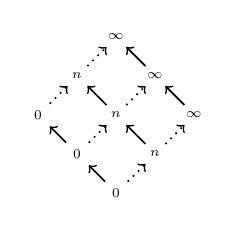
\begin{tikzpicture}
    [->,auto,semithick, every node/.style={scale=0.7}]
    \node(U) {$\kun_0$} ;
    \node(A) [above left of=U] {$\kaff_0$} ;
    \node(L) [above left of=A] {$\klin_0$} ;
    \node(Un) [above right of=U] {$\kun_n$} ;
    \node(An) [above left of=Un] {$\kaff_n$} ;
    \node(Ln) [above left of=An] {$\klin_n$} ;
    \node(Uinf) [above right of=Un] {$\kun_\infty$} ;
    \node(Ainf) [above left of=Uinf] {$\kaff_\infty$} ;
    \node(Linf) [above left of=Ainf] {$\klin_\infty$} ;
    \path
    (U) edge (A)
    (A) edge (L)
    (Un) edge (An)
    (An) edge (Ln)
    (Uinf) edge (Ainf)
    (Ainf) edge (Linf)
    ;
    \path[dotted]
    (U) edge (Un)
    (A) edge (An)
    (L) edge (Ln)
    (Un) edge (Uinf)
    (An) edge (Ainf)
    (Ln) edge (Linf)
    ;
  \end{tikzpicture}
\end{minipage}

%%% Local Variables:
%%% mode: latex
%%% TeX-master: "../main"
%%% End:

  % \caption{Lattice inequalities -- $k \lk_\Lat k'$}
  \begin{mathpar}
  \inferrule
  {}{ \entail{}{\Cleq{\kvar}{\kaff}} }
  \and
  \inferrule
  {}{ \entail{}{\Cleq{\kun}{\kvar}} }
  \and
  \inferrule
  {}{ \entail{}{\Cleq{\kvar}{\kvar}} }
  \and
  % \inferrule
  % {\Cleq{k}{k'} \in C}{ \entail{C}{\Cleq{k}{k'}} }
  % \and
  % \inferrule
  % { \entail{C}{\Cleq{x_1}{x}}\\
  %   \entail{C}{\Cleq{x}{x_2}}
  % }
  % { \entail{C}{\Cleq{x_1}{x_2}} }
  % \and
  % \inferrule
  % { \entail{C}{D} }
  % { \entail{C}{\Cproj{x}{D}} }
  % \\
  \inferrule
  { \entail{C}{\Cleq{\tau'_1}{\tau_1}}\\
    \entail{C}{\Cleq{\tau_2}{\tau'_2}}\\
    \entail{C}{\Cleq{k}{k'}}
  }
  { \entail{C}{\Cleq{\tau_1\tarr{k}\tau_2}{\tau'_1\tarr{k'}\tau'_2}} }
  \and
  \inferrule
  { \forall i,\ \entail{C}{\Cleq{\tau_i}{\tau_i}}\\
  }
  { \entail{C}{\Cleq{\tapp{t}{(\tau_i)}}{\tapp{t}{(\tau'_i)}}} }
  \and
  
  % \and
  % \inferrule
  % { \entail{C}{\Cleq{k}{k'}} \\
  %   \entail{C}{\Cleq{k'}{k}} }
  % { \entail{C}{\Ceq{k}{k'}} }
  % \and
  % \inferrule
  % { \entail{C}{\Cleq{k}{k'}} }
  % { \entail{C}{\Ckind{\tau_0\tarr{k}\tau_1}}{k'}}
  % \and
  % \text{Completion to form a cylindric constraint system.}
\end{mathpar}

%%% Local Variables:
%%% mode: latex
%%% TeX-master: "../main"
%%% End:

  \caption{Base entailment rules -- $\entail{\inP{C}}{\inP{D}}$ }
  \label{rules:entail}
\end{figure}

Let $\CL$ be the set of constraints in such a lattice $\mathcal L$.
The full grammar of constraints is shown in \cref{grammar:constraint}.
Constraints are made of kind inequalities, conjunctions and
projections along with type unification
constraints. Since types might contain kinds (for instance, on the arrows),
type unification is oriented and written as $\leq$.
For simplicity, we consider all type constructors
invariant in their parameters
and define $\Ceq{\tau}{\tau'}$ as $\Cleq{\tau}{\tau'} \wedge \Cleq{\tau'}{\tau}$.

Entailment is denoted by $\entail{C}{D}$,
where $D$ is a consequence of the constraints $C$.
We say that $C$ and $D$ are equivalent, $C \equivC D$,
when $\entail{C}{D}$ and $\entail{D}{C}$.
% The base rules for entailment are given in \cref{rules:entail}.
% The rules for classic Herbrand unification and
% projection operators are omitted for brevity (see
% \citep{DBLP:journals/tapos/OderskySW99} for
% details).
%

We directly reuse the following definitions from \hmx.

\begin{property}[Cylindric constraint system]
  A cylindric constraint system is a constraint system
  such that, for any constraint $C$:
\begin{align*}
  \entail{C&}{\Cproj{x}{C}}
  &\entail{C}{D} &\implies \entail{\Cproj{x}C}{\Cproj{x}D}\\
  \Cproj{x}{(C\wedge \Cproj{x}D)}&\equivC \Cproj{x}{C} \wedge \Cproj{x}D
  & \Cproj{x}{\Cproj{y}D}&\equivC \Cproj{y}{\Cproj{x}D}
\end{align*}
\end{property}

\begin{property}[Term rewriting system]
A term rewriting system is a system where, for every
types $\tau$,$\tau'$, there exists an equality predicates $\Ceq{\tau}{\tau'}$
which is symmetric, reflexive, transitive, stable under substitution and such that,
for any predicate $P$:
\begin{align*}
  &\entail{\Ceq{x}{y}\wedge \Cproj{x}C \wedge \Ceq{x}{y}}{C}\\
  &\subst{x}{\tau}{P} \equivC \Cproj{x}P \wedge \Ceq{x}{\tau}
                        \text{ where } x\notin\fv{\tau}
\end{align*}
\end{property}

\begin{definition}[Constraint system with lattice]
$\CL$ is defined as the smallest cylindric term constraint system that
satisfies the axiom shown in \cref{rules:entail}.
\end{definition}

% \begin{figure*}[!bt]
%   \centering
%   \begin{minipage}{0.32\linewidth}
%     \begin{align*}
%       C &::=  C_1 \Cand C_2  \tag{Conjunction}\\
%         &\mid \Cleq{\tau_1}{\tau_2} \mid \Cleq{k_1}{k_2} \tag{Inequalities} \\
%         &\mid \Cproj{\tvar}{C}
%         \mid \Cproj{\kvar}{C} \tag{Projections}
%     \end{align*}
%     \caption{The constraint language}
%     \label{grammar:constraint}
%   \end{minipage}\hfill
%   \begin{minipage}{0.66\linewidth}
%     \begin{mathpar}
%       \inferrule
%       {\forall i,\ \entail{C}{\Cleq{l_i}{k}}}
%       {\entail{C}{\Cleq{\wedge_i l_i}{k}}}
%       \and
%       \inferrule
%       {\forall i,\ \entail{C}{\Cleq{k}{l_i}}}
%       {\entail{C}{\Cleq{k}{\vee_i l_i}}}
%       \and
%       \inferrule
%       { \forall i,\ \entail{C}{\Ceq{\tau_i}{\tau_i}}\\
%       }
%       { \entail{C}{\Cleq{\tapp{\tcon}{(\tau_i)}}{\tapp{\tcon}{(\tau'_i)}}} }
%       \and
%       \inferrule{l \lk_\Lat l'}{\entail{}{\Cleq{l}{l'}}}
%       \and
%       \inferrule
%       { \entail{C}{\Cleq{\tau'_1}{\tau_1}}\\
%         \entail{C}{\Cleq{\tau_2}{\tau'_2}}\\
%         \entail{C}{\Cleq{k}{k'}}
%       }
%       { \entail{C}{\Cleq{\tau_1\tarr{k}\tau_2}{\tau'_1\tarr{k'}\tau'_2}} }
%     \end{mathpar}
%     \caption{Base entailment rules -- $\entail{\inP{C}}{\inP{D}}$ }
%     \label{rules:entail}
%   \end{minipage}
% \end{figure*}

We define the set of solved formed
$\mathcal S$ as the quotient set of $\CL$ by $\equivC$.
We will show later that such constraints are in fact only composed of
kind inequalities, and thus correspond to the syntactic constraints
used in type and kind schemes.
%
We now define our normalization procedure $\normalize{C_0}{\unif_0}$, where
$C_0\in \CL$ is a set of constraints and $\unif_0$ is a substitution.
It returns a constraint $C \in \mathcal S$ in
solved form and a unifier $\unif$.
The main idea of the algorithm is to first remove all the type equalities
by using regular Herbrand unification. After that, we only have
a set of inequalities among kinds, which we can consider as a relation.
We can then saturate the relation,
unify all kinds that are in the same equivalence classes to obtain
a most general unifier on kind variables,
remove all existentially quantified variables and
then minimize back the relation and apply various
simplification rules to make the resulting type easier to understand to users.

More precisely, we apply the following steps:
\begin{enumerate}
\item Solve all type equality constraints through Herbrand unification and
  gather all existential quantifications at the front of the constraint.
  We obtain a constraint $C^k = \exists \Multi\kvar,\ \Cleq{k_j}{k'_j}_j$ and
  a substitution $\unif_\tau$.

  We write $\mathcal R$ for the relation $\Cleq{k_j}{k'_j}_j$,
  $\mathcal G$ the underlying directed graph and $V$ its vertices.

\item Saturate the lattice equalities in $\mathcal R$.

  More precisely, for each kind variable $\kvar \in V$,
  for each constant $l_i$ (resp. $l_j$) such that
  there is a path from $l_i$ to $\kvar$ (resp. from $\kvar$ to $l_j$) in $\mathcal G$,
  add an edge from $\lub l_i$ to $\kvar$
  (resp. from $\kvar$ to $\glb l_j$).
  This step is well defined since $\mathcal L$ is a bounded lattice
  and $\lub\emptyset$ and $\glb\emptyset$ are well defined.

  We also complement $\mathcal R$ with $(\leq)$ by adding an edge
  between related constants.
\item
  At this point, we can easily check for satisfiability: A constraint
  is satisfiable (in the given environment) if and only if,
  for any constants $l_1$ and $l_2$ such that
  there is a path from $l_1$ to $l_2$ in $\mathcal G$, then $l_1\lk_\Lat l_2$.
  If this is not the case, we return \textbf{fail}.

\item For each strongly connected component in $\mathcal G$, unify all its vertices and replace it by a representative.
  We write $\unif_k$ for the substitution that replaces a kind variable by
  its representative.
  The representative of a strongly connected component $g$ can be determined as follows:
  \begin{itemize}
  \item If $g$ does not contain any constant, then the representative
    is a fresh kind variable.
  \item If $g$ contains exactly one constant, it is the representative.
  \item Otherwise, the initial constraint $C_0$ is not satisfiable.
  \end{itemize}
  Note that this step will also detect all unsatisfiable constraints.
\item Take the transitive closure of $\mathcal R$.
\item Remove all the vertices corresponding to the kind variables $\Multi\kvar$
  that are existentially quantified in $C^k$.
\item Take the transitive reduction of $\mathcal R$.
\item Remove the extremums of $\mathcal L$ and the edges of $(\leq)$
  from $\mathcal R$.
\item Return $C = \left\{ k \leq k' \mid k \operatorname{\mathcal R}k' \right\}$
  and $\unif =  \unif_\tau \meet \unif_k$.
\end{enumerate}

An example of this algorithm in action is shown in \cref{solving:example}.
Our algorithm is complete, computes principal normal forms,
and already simplifies constraints significantly
(thanks to steps 6, 7 and 8).
It can be extended with further simplification phases.
In particular, our implementation and all the signatures presented in
\cref{motivation} use a variance-based simplification
where all covariant (resp. contravariant) variables are replaced by their
lower (resp. upper) bounds.
All the simplification mechanisms presented
here, including the variance-based one, are complete.
It is also possible to add ``best-effort'' simplification
rules which help reduce the size of inferred signatures even further
\citep{DBLP:conf/aplas/Simonet03}.

% \subsection{Example of constraint solving and simplification}
% \label{solving:example}

% \label{solving:example}

\begin{figure}[tbp]
  \centering
  \begin{tikzpicture}[node distance=6mm,xscale=1.2,yscale=0.7,.every edge/.style=[link,->,>=latex,thick]]
    \node (U) {$\kun$} ;
    \node[above left=of U] (x) {$\kvar_x$} ;
    \node[above=of x] (r) {$\kvar_r$};
    \node[left=of x] (g) {$\kvar_\gamma$} ;
    \node[right=of x] (b) {$\kvar_\beta$} ;
    \node[right=of b] (3) {$\kvar_3$} ;
    \node[above=of 3] (f) {$\kvar_f$} ;
    \node[above=of f] (1) {$\kvar_1$} ;

    \draw (x) to[bend right] (U) ;
    \draw (x) -> (r) ;
    \draw (b) -> (r) ;
    \draw (g) -> (x) ;
    \draw (3) -> (f) ;
    \draw (f) -> (1) ;

    \draw[blue] (3) to[bend right] (1);

    \node at (-0.5,-0.5) {Before};
    
    \begin{scope}[dashed,gray]
      \draw (U) to[bend right] (x) ;
      \draw (U) to (b) ;
      \draw (U) to[bend left] (g) ;
      \draw (U) to (r) ;
      \draw (U) to (1) ;
      \draw (U) to (3) ;
      \draw (U) to (f) ;
    \end{scope}
  
    \begin{scope}[on background layer]
      \node[fill=green!20,draw=green,
      inner sep=-1pt,ellipse,rotate fit=-20,fit=(U.south) (x) (g)] {};
      \node[fill=red!20,draw=red, inner sep=-2pt, circle,fit=(r)] {};
      \node[fill=red!20,draw=red, inner sep=-2pt, circle,fit=(f)] {};
    \end{scope}
  \end{tikzpicture}~
  \vrule~
  \begin{tikzpicture}[node distance=7mm,every edge/.style=[link,->,>=latex,thick]]
    \node (b) {$\kvar_\beta$} ;
    \node[right=of b] (3) {$\kvar_3$} ;
    \node[above=of 3] (f) {} ;
    \node[above=of f] (1) {$\kvar_1$} ;

    \draw (3) to[bend right] (1);

    \node at (0.5,-1.5) {After};
  \end{tikzpicture}
  \vspace{-5pt}
    \caption{Graph representing the example constraints}
    \label{example:graph}
    % \caption{Final state of the graph}
    \label{example:graph:final}
\end{figure}

Consider the expression $\lam{f}{\lam{x}{(\app{f}{x},x)}}$.
The inference algorithm yields the following constraints:
%
\begin{align*}
  \E &= (\tvar_f : \kvar_f)
  (\tvar_x : \kvar_x)\dots\\
  C &= (\tvar_f \leq \gamma \tarr{\kvar_1} \beta )
  \Cand
  (\gamma \leq \tvar_x)
  \Cand
  (\beta \times  \tvar_x \leq \alpha_r)
  \Cand
  (\kvar_x \leq \kun)
\end{align*}

The first step of the algorithm uses Herbrand unification to obtain
a type skeleton. 
$$
(\gamma \tarr{\kvar_3} \beta) \tarr{\kvar_2} \gamma \tarr{\kvar_1} \beta \times  \gamma$$

In addition, we obtain the following kind constraints: 
\[\begin{aligned}
    % \Cproj{\kvar_r}\Cproj{\kvar_f}\Cproj{\kvar_x}{}
    &(\kvar_x \leq \kun)
    \Cand
    (\kvar_\gamma \leq \kvar_x)
    \Cand
    (\kvar_x \leq \kvar_r)
    \Cand
    (\kvar_\beta \leq \kvar_r)
    \Cand
    (\kvar_3 \leq \kvar_f)
    \Cand
    (\kvar_f \leq \kvar_1)
\end{aligned}\]
% Since $\kvar_r$, $\kvar_f$ and $\kvar_x$ are not present in the type skeleton,
% they are existentially quantified.

We translate these constraints into a relation whose graph
is shown in \cref{example:graph}.
%
The algorithm then proceeds as follow:
\begin{itemize}[noitemsep]
\item From the constraints above, we deduce the graph shown
  with plain arrows on the left of \cref{example:graph}.
\item We add all the dashed arrows by saturating
  lattice inequalities. For clarity, we only show $\kun$.
\item We identify the connected component circled in
  {\color{ForestGreen} green}.
  We deduce $\kvar_\gamma = \kvar_x = \kun$.
\item We take the transitive closure, which adds the
  arrow in {\color{blue} blue} from $\kvar_3$ to $\kvar_1$.
\item We remove the remaining nodes not present in the type skeleton (colored in {\color{red} red}): $\kvar_r$ and $\kvar_f$.
\item We clean up the graph (transitive reduction, remove unneeded constants, \dots),
  and obtain the graph shown on the right.
  We deduce $\kvar_3 \leq \kvar_1$.
\end{itemize}

The final constraint is thus
$$\kvar_\gamma = \kvar_x = \kun \Cand \kvar_3 \leq \kvar_1$$
If we were to generalize, we would obtain the type scheme:
$$\forall \kvar_\beta \kvar_1 \kvar_2 \kvar_3
(\gamma : \kun) (\beta : \kvar_\beta).\ %
\qual
{\Cleq{\kvar_3}{\kvar_1}}
{(\gamma \tarr{\kvar_3} \beta) \tarr{\kvar_2} \gamma \tarr{\kvar_1} \beta \times  \gamma}$$

We can further simplify this type by exploiting variance. As $\kvar_1$
and $\kvar_2$ are only used in covariant position, they can be
replaced by their lower bounds, $\kvar_3$ and $\kun$. 
By removing the unused quantifiers, we obtain a much simplified equivalent type:
$$
\forall \kvar
(\gamma : \kun).
{(\gamma \tarr{\kvar} \beta) \tarr{} \gamma \tarr{\kvar} \beta \times  \gamma}$$



%%% Local Variables:
%%% mode: latex
%%% TeX-master: "../main"
%%% End:


\subsection{Principal constraint system}

We now prove that $\CL$ supports all the properties necessary for
principal type inference, as defined by \hmx.
We first prove that constraint solving
does compute normal forms, and that such normal forms are unique.


\begin{lemma}[Principal normal form]
  \label{lemma:normalform}
  Given a constraint $D\in\CL$, a substitution $\phi$ and
  $(C,\unif) = \normalize{D}{\phi}$,
  then $\phi\leq\unif$,
  $C \equivC \unif D$ and
  $\unif C = C$.
\end{lemma}
\begin{proof}
  % For simplicity, we assume that any substitution has been already applied
  % to $D$ and that $\phi = id$.
  Let us partition $\phi$ into a part which affects type variables,
  $\phi_\tau$, and a part which affects kind variables, $\phi_k$.

  We write $(C^k,\unif_\tau)$ for the result of
  the modified Herbrand unification on $(D,\phi)$ in step (1).
  Herbrand unification computes the most general
  unifier. Our modified Herbrand unification only output additional
  kind constraints for kind on the arrows and does not change
  the result of the unification. Thus, we have
  $\phi_\tau\leq\unif_\tau$,
  $C^k \equivC \unif_\tau D$ and
  $\unif_\tau C^k = C^k$.

  Let $C^{k+}$ be the result after step (2), we trivially have that
  $\fv{C^{k+}} = \fv{C^k}$ and that $C^{k+} \equivC C^k$.

  Let $C^{A}$ and $\unif_k$ be the results after step (4).
  By definition, we have $\unif_k C^{k+} \equivC C^{A}$ and
  $\unif_k C^{A} = C^{A}$. Since $\phi_k$ has already be applied to $C$ before
  unifying the strongly connected components,
  we have that $\phi_k\leq\unif_k$.

  Let $\unif = \unif_\tau \meet \unif_k$. Since $\unif_\tau$ and $\unif_k$
  have disjoint supports,
  we have $C^{A} = \unif_\tau C^{A} \equivC \unif C^{k+} \equivC \unif D$
  and $\unif C^{A} = C^{A}$.
  Furthermore, $\phi_\tau \meet \phi_k \leq \unif_\tau \meet \unif_k$.

  Steps (5) to (9) all preserve the free variables and the equivalence
  of constraints, which concludes.
\end{proof}

\begin{lemma}[Uniqueness]
  Given $(C_1,\unif_1)$ and $(C_2,\unif_2)$ such that
  $\unif_1 C_1 \equivC \unif_2 C_2$,\\
  then
  $\normalize{C_1}{\unif_1}$ and $\normalize{C_2}{\unif_2}$
  are identical up to $\alpha$-renaming.
\end{lemma}
\begin{proof}
  In \cref{lemma:normalform}, we have showed that all the steps of the
  normalization procedure preserve equivalence.
  Since $\unif_1 C_1 \equivC \unif_2 C_2$, equivalence between
  the two results of the normalization procedures is preserved for all steps.

  We write $P(C_a)$ if for all $C = (k, k)'$
  such that $\entail{C_a}{C}$ and $\nvdash_eC$,
  we have $C \in {\mathcal R}_a$.

  Let us write $C_1'$ and $C_2'$ for the constraints after step (4). $P(C_1')$ and
  $P(C_2')$ hold. Indeed, since $C_1'$ and $C_2'$ are only composed
  of existential quantifications and kind inequalities, the only rules
  that applies are transitivity and lattice inequalities.
  After step (2) and (5), the associated relations are fully saturated for these
  two rules, hence all inequalities that can be deduced from $C_a'$ are already
  present in the relation.

  The property $P$ is preserved by step (6) since we only remove
  inequalities that involve existentially quantified variables. Such
  inequalities could not be picked in $P$.
  % In (6) we only remove
  % trivial lattice inequalities.

  Let us write $C''_a$ for $a\in\{1,2\}$ the constraints after step (5).
  Since there are no more existential variables,
  we have $C''_a=(k_i,k'_i)_i=\mathcal R''_a$.
  For any $C=(k,k')$ such that $\entail{}{C}$ and $\entail{C''_a}{C}$,
  then $C \in (\leq) \subset {\mathcal R}''_a$.
  Indeed, the only trivial inequalities in our system are equalities of the form
  $(\kvar, \kvar)$, which were removed in step (4) and the lattice inequalities.

  Let us consider $C = (k,k') \in \mathcal R''_1$.
  Since $C''_1\equivC C''_2$, we have $\entail{C''_2}{C}$.
  If $\nvdash_e{C}$, by $P(C''_2)$ we have that
  $C\in R''_2$.
  If $\entail{}{C}$, then $C\in (\leq) \subset R''_2$.
  We conclude that $R''_1 \subset R''_2$.
  By symmetry, $R''_1 = R''_2$ and $C''_1 = C''_2$.

  This equality is preserved by step (7) and (8)
  since the transitive reduction of a directed acyclic graph is unique,
  which concludes.
\end{proof}

We can now prove all the necessary high level properties.

\begin{lemma}
  For all $C\in\mathcal S$, $\entail{C}{x = x}$ implies
  $\entail{}{x = x}$.
\end{lemma}
\begin{proof}
  By definition of $\operatorname{normalize}$, We have $C = \Multi{\Cleq{k}{k'}}$
  such that the underlying relation has no cycles.
  Thus, we can not deduce neither kind nor type equalities from $C$.
\end{proof}

\begin{property}[Regular constraint system]
  $\CL$ is regular, ie, for $x, x'$ two types or kinds,
  $\entail{}{\Ceq{x}{x'}}$ implies
  $\fv{x} = \fv{x'}$
\end{property}
\begin{proof}
  The only equalities possibles are between variables (via symmetry) or
  between constants.
\end{proof}

Finally, we can conclude with all the properties we need for
\hmx:

\begin{theorem}[Principal constraints]
  $\CL$ has the principal constraint property,\\
  $\operatorname{normalize}$ computes principal normal forms for $\CL$
  and $\CL$ is regular.
\end{theorem}


This is sufficient to show that $HM(\CL)$ is principal. However,
we do not use \hmx directly but an extended version with kind inference,
linear and affine types, and borrow.
We extend the proofs of \hmx to such a system in \cref{appendix:infer}.


\section{Syntax-directed typing}
\label{appendix:sdtyping}

\begin{figure}[bt]
  \centering
  \begin{mathpar}
  \inferrule[KVar]
  { \bvar{\tvar}{k} \in \E }
  { \inferSK{C}{\E}{\tvar}{k}
  }
  \and
  \inferrule[KPair]
  { \forall i \quad
    \inferSK{C}{\E}{\tau_i}{k_i} \quad
    \inferSS{C}{\E}{k_i}{k}
  }
  { \inferSK{C}{\E}{\tyPair{\tau_1}{\tau_2}}{k} }
  \and
  \inferrule[KApp]
  { \bvar{\T{\tcon}}{
      \forall \Multi[i]\kvar.\ \qual{D}{(\Multi[j]{k'}) \karr k'}}
    \in \E \\
    \unif = \subst{\Multi[i]\kvar}{\Multi[i]k}{} \\
    \entail C {\unif D} \\
    \forall j\quad
    \inferSK{C}{\E}{\tau_j}{k_j}\quad
    \inferSS{C}{\E}{k_j}{\unif{k'_j}}
  }
  { \inferSK{C}{\E}{\tapp{\tcon}{\Multi[j]{\tau}}}{\unif{k'}} }
  \and
  \inferrule[KBorrow]
  {}{ \inferSK{C}{\E}{\borrowty{k}{\tau}}{k}}
  \and
  \inferrule[KArr]
  {}
  { \inferSK{C}{\E}{\tau_1 \tarr{k} \tau_2}{k} }
\end{mathpar}


%%% Local Variables:
%%% mode: latex
%%% TeX-master: "../main"
%%% End:

  \caption{Syntax-directed kinding rule --
    $\inferSK{C}{\E}{\tau}{k}$}
  \label{rules:sd-kinding}
\end{figure}

\begin{figure}[!tbp]
  \begin{mathpar}
  \inferrule[ESplit-Empty]{}{
    \bsplit{\Cempty}\Eempty\Eempty\Eempty
  }

  \inferrule[ESplit-Nonempty]{
    \bsplit{C_1}{\E}{\E_1}{\E_2} \\
    \bsplit{C_2}{b}{b_1}{b_2}
  }{
    \bsplit{C_1\Cand C_2}{\E;b}{\E_1;b_1}{\E_2;b_2}
  }

  \inferrule[ESplit-Check]{
    \bsplit{D}{\E}{\E_1}{\E_2} \\
    \entail{C}{D}
  }{
    \lsplit{C}{\E}{\E_1}{\E_2}
  }
\end{mathpar}
\hrulefill
\begin{mathpar}
  \inferrule[BSplit-Both]{}{
    \bsplit {\Cleq{\schm}{\kun_\infty}}
    {\bvar{x}{\schm}} {\bvar{x}{\schm}} {\bvar{x}{\schm}}
  }

  \inferrule[BSplit-Left]{}{
    \bsplit {\Cempty} {\bvar{x}{\schm}} {\bvar{x}{\schm}} {\bnone}
  }

  \inferrule[BSplit-Right]{}{
    \bsplit {\Cempty} {\bvar{x}{\schm}} {\bnone} {\bvar{x}{\schm}}
  }

  \inferrule[BSplit-Imm-Borrow]{}{
    \bsplit {\Cempty}
    {\bvar{\borrow[\IBORROW]{x}}{\schm}}
    {\bvar{\borrow[\IBORROW]{x}}{\schm}}{\bvar{\borrow[\IBORROW]{x}}{\schm}}
  }

  \inferrule[BSplit-To-Borrow]{}{
    \bsplit {\Cempty}{\bvar x \schm}{\svar x \schm^n}{\bvar x \schm}
  }

  \inferrule[BSplit-To-Imm]{}{
    \bsplit {\Cempty}
    {\bvar{\borrow x} \schm}{\svar[\IBORROW] x \schm^n}{\bvar{\borrow x} \schm}
  }
\end{mathpar}
%%% Local Variables:
%%% mode: latex
%%% TeX-master: "../main"
%%% End:

  \caption{Splitting ---
    environments $\lsplit C\E{\E_l}{\E_r}$;
    inference $\bsplit C\E{\inP{\E_l}}{\inP{\E_r}}$;
    binders $\bsplit Cb{\inP{b_r}}{\inP{b_l}}$}
  \label{fig:sd-splitting}
\end{figure}
\begin{figure}[!tbp]
  \begin{mathpar}
  \inferrule[EBorrow]{
    \bregion{C_r}{}{\svar{x}{\tau}^n}{b}
  }{
    \bregion{C_r}{x}{\E;\svar{x}{\tau}^n}{\E; b}
  }

  \inferrule[EBorrow-Check]{
    \entail{C}{D}\\\\
    \bregion{D}{x}{\E;\svar{x}{\tau}^n}{\E; b}
  }{
    \lregion{C}{x}{\E;\svar{x}{\tau}^n}{\E; b}
  }
  
  \inferrule[EBorrow-Binder]{
    \BORROW\in\left\{\kun,\kaff\right\}\\
    C = (\BORROW_n\lk k) \wedge (k \lk \BORROW_\infty)
  }{
    \bregion{C}{}
    {\svar[\BORROW]{x}{\tau}^n}
    {\bvar{\borrow[\BORROW]{x}}{\borrowty[\BORROW] k{\tau}}}
  }
\end{mathpar}
%%% Local Variables:
%%% mode: latex
%%% TeX-master: "../main"
%%% End:

  \caption{Borrowing ---
    environments $\lregion[n]{C}{x}{\E}{\E'}$;
    inference $\bregion[\inP n]{C}{\inP x}{\E}{\inP{\E'}}$;
    binders $\bregion[\inP n]{C}{\inP x}{b}{\inP{b'}}$}
  \label{fig:sd-borrowing}
\end{figure}
\begin{figure*}[tbp]
  \begin{mathpar}
  \inferrule{}{ \Cleq{\Eempty}{k} \Crewrite  \Cempty}

  \inferrule{
    \Cleq\E k \Crewrite  C \\ \E \vdash \Cleq B k \Crewrite  D
  }{
    \Cleq{\E; B}{k} \Crewrite  C \Cand D
  }
  \\
  \inferrule{
    \E \vdash \Cleq \schm k \Crewrite  C
  }{ \E \vdash \Cleq{\bvar x \schm}{k} \Crewrite  C}

  \inferrule{
    \E \vdash \Cleq \schm k \Crewrite  C \\
    \Cleq{\BORROW^n} k  \Crewrite  D
  }{
    \E \vdash \Cleq{\svar x \schm^n} k \Crewrite  C \Cand D
  }
  \\
  \inferrule{}{\Cleq{\IBORROW^n} k \Crewrite  \Cleq{\kun_n} k}

  \inferrule{}{\Cleq{\MBORROW^n} k \Crewrite  \Cleq{\kaff_n} k}
  \\
  \inferrule{
    \E; \Multi{\bvar{\alpha}{k}} \vdash \Cleq\tau k \Crewrite  D
  }{
    \E \vdash \Cleq{\forall\Multi\kvar\forall\Multi{\bvar{\alpha}{k}}.(\qual{C}{\tau})}
    k \Crewrite  C \Cand D
  }

  \inferrule{}
  { \E \vdash \Cleq{ \tau_2\tarr{k'}\tau_1 } k \Crewrite  \Cleq{k'}k }

  \inferrule{
    \E(\tvar) = \kschm
  }
  { \E \vdash \Cleq{ \tvar} k \Crewrite  \Cleq\kschm k }

  \inferrule{
  }{ \E \vdash \Cleq{\tapp{t}{\Multi\tau}} k \Crewrite  ???}

  \inferrule{}{
    \E \vdash \Cleq{\borrowty {k'} {\tau}} k \Crewrite  \Cleq{k'}k
  }
\end{mathpar}

%%% Local Variables:
%%% mode: latex
%%% TeX-master: "../main"
%%% End:

  \caption{Rewriting constraints on environments --- $\inP{\Cleq{\E}{k}}\Crewrite  C$}
  \label{fig:contraints-environments-types}
% \end{figure*}
% \begin{figure*}[!tbp]
  \begin{mathpar}
  \inferrule[Scheme]{
    \inferSK{C \Cand C_x} \E \tau {k'} \\
    \entail C {\Cleq{k'}k}
  }{
    \entail C {(\forall \kvar_i \forall (\tvar_j:k_j).\
      \qual{C_x}{\tau}) \le  k}
  }
\end{mathpar}
\hrulefill
\begin{mathpar}
  \inferrule[Var]
  { \bvar{x}{
      \forall \kvar_i \forall (\tvar_j:k_j).\ \qual{C_x}{\tau}
    }
    \in \E \\
    \unif = [\kvar_i\mapsto k_i,\tvar_j \mapsto \tau_j] \\
    \entail C {\unif(C_x)} \\
    % \addlin{
    %   \inferSK{C}{\E}{\unif \tau}{k_\tau}
    % }
  }
  { \inferS{C}{\E}{x}{\unif\tau}
  }
  \and
  \ruleSDLam
  \and
  \ruleSDApp
  \and
  \inferrule[Let]
  { \inferS{C \Cand D}{\E_1}{e_1}{\tau_1} \\
    \schm = \forall\Multi\kvar\forall\bvar{\Multi\tvar}{\Multi{
        k}}. \qual{D}{\tau_1}\\
    \{\Multi\kvar, \Multi\tvar\} = \fv{D, \tau_1} \setminus \fv{C, \E}
  \\
  \entail{C}{\exists\Multi\kvar\Multi\tvar.D} \\
    \inferS{C}{\E;\bvar{x}{\sigma}}{e_2}{\tau_2} \\
    \addlin{\lsplit{C}{\E}{\E_1}{\E_2}}\\
  }
  { \inferS{C}
    {\E}{\letin{x}{e_1}{e_2}}{\tau_2} }
  \and
  \inferrule[Pair]
  { \inferS{C}{\E_1}{e_1}{\tau_1} \\
    \inferS{C}{\E_2}{e_2}{\tau_2} \\
    \addlin{\lsplit{C}{\E}{\E_1}{\E_2}}
  }
  { \inferS{C}{\E}{\introPair{e_1}{e_2}}{\tyPair{\tau_1}{\tau_2}} }
  \and
  \inferrule[MatchPair]
  { 
    \inferS{C}{\E_1}{e_1}{\tyPair{\tau_1}{\tau'_1}} \\
    \inferS{C}
    {\E_2;\bvar{x}{\tau_1};\bvar{x'}{\tau'_1}}{e_2}{\tau_2} \\
    \addlin{\lsplit{C}{\E}{\E_1}{\E_2}}
  }
  { \inferS{C}
    {\E}{\matchin{x,x'}{e_1}{e_2}}{\tau_2} }
  \and
  %
  \inferrule[Borrow]
  { 
    \bvar{\borrow x}{\borrowty k\tau} \in \E
  }
  { \inferS{C}{\E}{\borrow{x}}{\borrowty{k}{\tau}} }
  \and
  \inferrule[Region]
  { \svar x {\tau_x} \in \E \\
    \addlin{ \bregion{C_r}{x}{\E}{\E'} }\\
    \inferS{C}{\E'}{e}{\tau} \\
    \inferSK{C}{\E}{\tau}{k_\tau}\\
    \entail C {\Cleq{k_\tau}{\klin_{n-1}}} \\
  }  { \inferS{C}{\E}{\region{x}{e}}{\tau} }
  \and
  %
  % \inferrule[Elim]
  % { \tvar,(\kvar'_i),(\tvar'_j)\text{ new}\\
  %   \bvar{K}{
  %     \forall \kvar_i \forall (\tvar_j:\kvar_j).\ \qual{C_K}{\tau_1 \tarr{}\tau_2}
  %   } \in \E\\
  %   \inferW{\Sv}{(C,\unif)}{\E}{e}{\tau} \\
  %   \unif' =
  %   \subst{\kvar_i}{\kvar'_i}{} \meet
  %   \subst{\tvar_j}{\tvar'_j}{} \meet \unif \\
  %   D =
  %   C \Cand C_K \Cand \Cleq{\tau_1}{\tvar} \Cand \Cleq{\tau}{\tau_2} \\
  %   (C,\unif) = \normalize{D}{\unif'}\\
  % }
  % { \inferW{\addlin{\Sv}}{(C,\unif|_{\fv{\E}})}{\E}{\elimK{K}{e}}
  %   {\unif\tvar} }
\end{mathpar}

% \begin{align*}
%   \Weaken(x,\Sv)
%   &\equiv \begin{cases}
%     \operatorname{kind}(x)\lk\kun &\text{if } \operatorname{kind}(x)\in\Sv\\
%     \Cempty &\text{otherwise}
%   \end{cases}\\
%   \Cleq{\Sv}{k}
%   &\equiv \bigwedge_{\kvar\in\Sv} \Cleq{\kvar}{k}
% \end{align*}

%%% Local Variables:
%%% mode: latex
%%% TeX-master: "../main"
%%% End:

  \caption{Syntax-directed typing rules --
    $\inferS{C}{\E}{e}{\tau}$}
  \label{fig:syntax-directed-typing}
\end{figure*}
\begin{figure*}[!btp]
  \begin{mathpar}
  \ruleSDIVar
  \and
  \ruleSDIVarInst
  \and
  \ruleSDIApp
  \and
  \ruleSDIPair
  \and
  \ruleSDILam
  \and
  \and
  \ruleSDILet
  \and
  \ruleSDIPLet
  \and
  \ruleSDIMatchPair
\end{mathpar}

%%% Local Variables:
%%% mode: latex
%%% TeX-master: "../main"
%%% End:

  \caption{Syntax-directed typing rules for internal language --
    $\inferS{C}{\E}{e}{\tau}$}
  \label{fig:syntax-directed-typing-internal}
\end{figure*}
% \begin{figure*}[!btp]
%   \begin{mathpar}
  % \ruleSDIVar
  % \and
  % \ruleSDIVarInst
  % \and
  \ruleSDAIApp
  \and
  \ruleSDAIPair
  \and
  % \ruleSDILam
  % \and
  % \ruleSDRegion
  % \and
  % \ruleSDConst
  % \and
  % \ruleSDBorrow
  % \and
  % \ruleSDReBorrow
  % \and
  % \ruleSDILet
  % \and
  % \ruleSDIPLet
  % \and
  \ruleSDAIMatchPair
  % \and
  % \ruleSDCreate
  % \and
  % \ruleSDObserve
  % \and
  % \ruleSDUpdate
  % \and
  % \ruleSDDestroy
\end{mathpar}

%%% Local Variables:
%%% mode: latex
%%% TeX-master: "../main"
%%% End:

%   \caption{Syntax-directed typing rules for internal language in A-normal form --
%     $\inferS{C}{\E}{e}{\tau}$}
%   \label{fig:syntax-directed-typing-internal-a}
% \end{figure*}

\subsection{Kinding}

We write $\inferSK{C}{\E}{\tau}{k}$
if $\tau$ has kind $k$ in environment $\E$ under constraints $C$.
The rules are shown in \cref{rules:sd-kinding}.
Kinds and types follow a small calculus with variables ($\tvar$,\dots),
functions (type constructors $\T{t}$), application ($\tapp{\tcon}{\Multi{\tau}}$)
and primitives such as types for arrows ($\tau\tarr{k}\tau'$) and
borrows ($\borrowty{k}{\tau}$).
Kind checking can thus be done in a fairly straightforward, syntax-directed
fashion by simply following
the syntax of the types. Kind arrows can only appear when looking
up the kind scheme of a type constructor $\T t$. Kind arrows are forbidden
in any other contexts.

\subsection{Environments}
\label{typ:extra:envs}

In \cref{sdtyping}, we only gave a partial description of
the splitting and borrowing relations on environments,
$\lsplit C\E\E\E$ and $\lregion C{x}\E\E$.
The complete definitions are shown on \cref{fig:sd-splitting,fig:sd-borrowing}.
All the definitions are made in term of the inference version, which
returns fresh constraints. The solving version then simply
uses entailment, as shown in rule {\sc ESplit-Check} and
{\sc EBorrow-Check}.
The remaining new rules are dedicated to iterating over the environment.

\cref{fig:contraints-environments-types} defines
the rewriting relation on environment constraints,
$\Cleq\E k \Crewrite C$, which rewrites a constraint of the form
$\Cleq\E k$ into $C$. It proceeds by iterating over the environment
and expanding the constraints for each binding.
Suspended bindings are rejected ({\sc ConstrSusp}).
Borrow bindings directly use the annotated kind ({\sc ConstrBorrow}).
Other bindings use the underlying type scheme ({\sc ConstrBinding}).
Type schemes are constrained by first inferring the kind, and then
emitting the constraint ({\sc ConstrSD} and {\sc ConstrI}).


\subsection{Typing}

The rules for syntax-directed typing are shown in \cref{fig:syntax-directed-typing}
and follow the presentation given in \cref{sdtyping}.
As usual in HM type systems, introduction of type-schemes
is included in the {\sc Let} rule via generalization.
We define $\generalize{C}{\E}{\tau} =
(\Cproj{\Multi{\kvar},\Multi{\tvar}}{C},
\forall \Multi{\kvar},\Multi{\tvar}.\qual{C}{\tau})$
where
$\Multi{\kvar},\Multi{\tvar} = (\fv{\tau}\cup\fv{C})\setminus\fv{\E}$.
The typing rules specific to the internal language are shown in
\cref{fig:syntax-directed-typing-internal}.
% The typing rules specific to the internal language in A-normal form are shown in
% \cref{fig:syntax-directed-typing-internal-a}.

%%% Local Variables:
%%% mode: latex
%%% TeX-master: "../main"
%%% End:
